   
        
        \begin{ledgroupsized}[r]{120mm}
        \footnotesize 
        \pstart        
        \noindent\textbf{\"{U}berlieferung:}  
        \pend
        \end{ledgroupsized}
      
       
              \begin{ledgroupsized}[r]{114mm}
              \footnotesize 
              \pstart \parindent -6mm
              \makebox[6mm][l]{\textit{L}}Konzept: LH XXXVIII Bl. 188. 1 Bl. 10 x 21 cm. 1 S. Oberer und unterer Seitenrand beschnitten. R\"{u}ckseite leer. Die beiden Zeichnungen links oben, Text umlaufend.\\Cc 2, Nr. 1554 \pend
              \end{ledgroupsized}
        %\normalsize
        \vspace*{5mm}
        \begin{ledgroup}
        \footnotesize 
        \pstart
      \noindent\footnotesize{\textbf{Datierungsgr\"{u}nde}: Die Datierung beruht auf dem letzten Satz des St\"{u}cks. Leibniz hat Tschirn\-haus Ende August 1675 in Paris kennengelernt, der ihm das Instrument offenbar w\"{a}hrend eines der gemeinsamen Arbeitstreffen gezeigt hat.}
        \pend
        \end{ledgroup}
      
        \vspace*{8mm}
        \pstart 
        \normalsize
      [188 r\textsuperscript{o}] \selectlanguage{ngerman}Instrument so einer im Sack tragen kan, und da dienet leicht zimbliche grosse gewicht, \edtext{zu ziehen. Ein mensch kan damit leicht etliche}{\lemma{gewicht,}\Afootnote{ \textit{ (1) }\ ja viele \textit{ (2) }\ zu [...] etliche \textit{ L}}} Zentner ziehen. Es bestehet aus 2 theilen \textit{A}, \textit{B} eines wie das andere ist ein Holz, iedes etwa 1 schuch lang, und deßen dicke etwa so das es zw\"{o}liff facen, oder seiten haben kann, in ieder seite plano, stehet ein rad oder trochlea\protect\index{Sachverzeichnis}{trochlea}, \edtext{eines so perpendicular}{\lemma{trochlea,}\Afootnote{ \textit{ (1) }\ so ihm perpendicular \textit{ (2) }\ eines so perpendicular \textit{ L}}} zu den selben plano, und durch den ganzen stab gehet auff der anderen seite wieder heraus; \edtext{die Trochleae\protect\index{Sachverzeichnis}{trochlea} als \textit{C}, \textit{D}}{\lemma{}\Afootnote{die Trochleae\protect\index{Sachverzeichnis}{trochlea} als \textit{C}, \textit{D} \textit{ erg.} \textit{ L}}} stehen also eines immer tieffer als das andere, das sie in ein ander nicht hindern denn mit einem faden \edtext{immer}{\lemma{}\Afootnote{immer \textbar\ alternis \textit{ gestr.}\ \textbar\ von \textit{ L}}} von den globen oder trochlea\protect\index{Sachverzeichnis}{trochlea} des einen \edtext{baculo}{\lemma{}\Afootnote{baculo \textit{ erg.} \textit{ L}}} zu den respondente des anderen; und folgends in eodem baculo von einer trochlea\protect\index{Sachverzeichnis}{trochlea} zu der n\"{a}chsten: ordinario more, so wird alsdann alles fertig seyn, das ende des fadens in den einen baculo ist daran fest, in den anderen gehet daraus und ist in die hand zu nehmen; an den baculum \edtext{daran}{\lemma{baculum}\Afootnote{ \textit{ (1) }\ so \textit{ (2) }\ daran \textit{ L}}} der faden fest, h\"{a}fftet man auch das \edtext{gewicht}{\lemma{das}\Afootnote{ \textit{ (1) }\ daran \textit{ (2) }\ gewicht \textit{ L}}} so man ziehen will, den anderen baculum macht man an einen orth f\"{a}st, und nimt den daran rausgehenden faden mit der Hand und ziehet daran; eine person kan gar leicht 6 personen an sich ziehen. Die krafft wird etwa 8 mahl vermehrt, dann wan 8 ellen des \edtext{fadens}{\lemma{des}\Afootnote{ \textit{ (1) }\ einen fad \textit{ (2) }\ fadens \textit{ L}}} mit der hand heraus gezogen ist etwa das gewicht umb eine elle gestiegen. Wann eine winde oder manivelle applicirt an den baculum, so schneidet der faden nicht die hand, und gewinnet man damit noch soviel kr\"{a}ffte als man fuglich begehren kan. Es ist der vortheil dabey, das instrument bey sich zu tragen; kr\"{a}fftig genugsam ad usum ordinarium; und gewißlich wunderlich den Leuten scheinet, und ihnen utilitatem matheseos gleich zu zeigen dienet. Mag etwa von einem teutschen handwergsman gefunden worden seyn. Es ist notabel dabey das die corden gar d\"{u}nne seyn k\"{o}nnen, und doch nicht reißen, als so 2 menschen ein massam sich zuziehen wie ein bindfaden; 6 menschen, wie ein kleines stricklein, sogar genug. Inventum forte cujusdam opificis Germanici, Herr Tschirnhaus\protect\index{Namensregister}{\textso{Tschirnhaus} (H.v.Tch., H.v.Tsch.), Ehrenfried Walther v. 1651\textendash 1708} hat es bey sich und mir gewießen.\selectlanguage{latin}
      \pend 
%\vspace{4.0ex}
%       \begin{center}
%       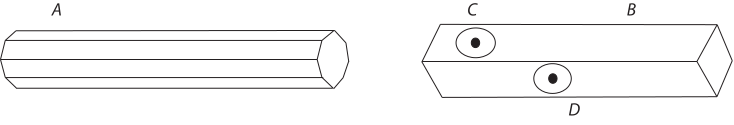
\includegraphics[width=1.0\textwidth]{images/38_188r1}
%       \\\textit{[Fig. 1]}\\
%       \vspace{3.0ex}
%       
\includegraphics[width=0.7\textwidth]{images/38_188r2}
%       \\\vspace{1.0ex}\textit{[Fig. 2]}\\
%       \end{center}